In order to maintain the configuration of the constellation for a longer time, a thruster is installed in each satellite to correct the decrease in altitude due to the orbit decay. The most optimal way to maintain the altitude is through a low-thrust maneuver. However, since this is a preliminar study, the calculations will be computed for a Hohmann transfer maneuver, which is simpler and more effective, but requires more propellant and greater increases of velocity. That is, by computing the velocity and propellant needed for a Hohmann maneuver, the results will be safe for a low-trust maneuver, because the late one requires less energy.

\subsubsection{Energy equation}
The deduction of the equations needed to solve the Hohmann maneuver begins with the energy equation:
\begin{equation}
\frac{V^2}{2}-\frac{\mu}{r}=-\frac{\mu}{2a}
\end{equation}
where $V$ is the orbital velocity of the satellite, $r$ is the distance from the focus, $a$ the semimajor axis of the orbit and $\mu$ the gravitational constant of the attracting body, in this case, the Earth. This expression shows that the total energy of the satellite equals the sum of its kinetic  and potential energy (per mass unit).
\paragraph{}
This equation can be arranged to obtain the velocity of the satellite. In the case of a circular orbit, the radius is constant, and equal to the semimajor axis. Replacing $a=r$ in the energy equation and after some operations, the expression of the velocity of a circular orbit is obtained:
\begin{equation}
V_{c}=\sqrt{\frac{\mu}{r}}
\end{equation}
\paragraph{}
As it can be deduced from the energy equation, a change in orbital velocity leads to a change in the value of the semimajor axis. This property is used in satellites to change their orbit through a velocity increment $\Delta V$. This process is called an orbital maneuver.

\subsubsection{Delta-V}
If the velocity increment $\Delta V$ is done instantaneously, the maneuver is called an impulsive maneuver. The Hohmann transfer is a two-impulse transfer between coplanar circular orbits. From an inicial circular orbit, a tangential velocity increment $\Delta V_{1}$ is applied to change the orbit to an ellipse. This ellipse is the transfer orbit, in which the perigee radius is the radius of the initial circular orbit and the apogee radius equals the radius of the final circular orbit. When the satellite reaches the apogee, a second velocity increment $\Delta V_{2}$ is applied, so that the satellite reaches the final circular orbit with the apogee radius. If this second velocity is not applied, the satellite will remain in the elliptic orbit.
\begin{figure}
\centerline{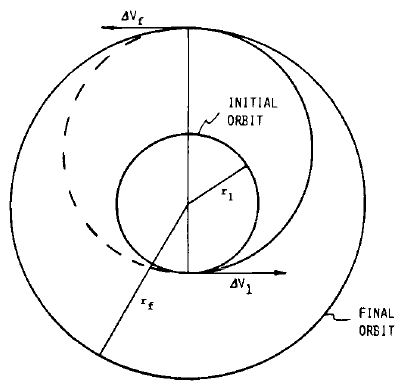
\includegraphics[scale=0.7]{ThrustersDrag/Hohmann.png}}
\caption{Hohmann transfer. Extracted from \cite{Chobotov2002}}
\end{figure}

With the energy equation defined above, it is easy to determine the velocity of the satellite in each orbit. The first orbit and the final ones are circular:
\begin{equation}
V_{1}=\sqrt{\frac{\mu}{r_{1}}}
\end{equation}
\begin{equation}
V_{f}=\sqrt{\frac{\mu}{r_{f}}}
\end{equation}
The velocity in the transfer orbit can be easily calculated with the energy equation applying the definition of the semimajor axis of an ellipse:
\begin{equation}
a=\frac{r_{1}+r_{f}}{2}
\end{equation}
The velocities in the perigee and apogee are:
\begin{equation}
V_{p}=\sqrt{\frac{2\mu r_{f}}{r_{1}(r_{1}+r_{f})}}
\end{equation}
\begin{equation}
V_{a}=\sqrt{\frac{2\mu r_{1}}{r_{f}(r_{1}+r_{f})}}
\end{equation}
Therefore the velocity increments are:
\begin{equation}
\Delta V_{1}=V_{p}-V_{1}=\sqrt{\frac{2\mu r_{f}}{r_{1}(r_{1}+r_{f})}}-\sqrt{\frac{\mu}{r_{1}}}
\end{equation}
\begin{equation}
\Delta V_{2}=V_{f}-V_{a}=\sqrt{\frac{\mu}{r_{f}}}-\sqrt{\frac{2\mu r_{1}}{r_{f}(r_{1}+r_{f})}}
\end{equation}

\subsubsection{Time}
It is also necessary to know the time needed to do the maneuver. This time is equal to half of the period of the transfer ellipse:
\begin{equation}
t=\frac{T}{2}=\frac{1}{2}\sqrt{\frac{4\pi^{2}a^{3}}{\mu}}
\end{equation}

\subsubsection{Propellant}
In order to know the mass of propellant needed in the maneuver, the Tsiolkovsky rocket equation is applied:
\begin{equation}
\Delta V=g_{0}I_{sp}\ln{\frac{m_{1}}{m_{f}}}=g_{0}I_{sp}\ln{\frac{m_{1}}{m_{1}-m_{prop}}}
\end{equation}
where $\Delta V=\Delta V_{1}+\Delta V_{2}$ is the total velocity increment of the maneuver, $g_{0}$ is the Earth's gravity, $I_{sp}$ is the specific impulse of the thruster used, $m_{1}$ is the initial mass of the satellite, $m_{f}$ is its final mass and $m_{prop}$ is the mass of propellant used in the maneuver.
\begin{equation}
m_{prop}=m_{1}\Bigg(1-\exp\bigg(-\frac{\Delta V}{g_{0}I_{sp}}\bigg)\Bigg)
\end{equation}

\subsubsection{Orbit maintenance}
As explained at the beggining of the section, the orbital maneuvers exposed are intented to maintain the altitude of the satellite for a longer time and, consequently, lengthen its life.
The method proposed begins when the satellite is deployed at a given height. This height will decrease due to the orbit decay, reaching a critical value, the limit altitude in which the constellation provides global coverage or another given height. Once this critical altitude is achieved, the satellite is put once again at its initial height through a Hohmann maneuver.
The process is repeated several times until the satellite runs out of propellant or until it reaches its desired lifetime.
\newline
In reality the satellite will perform a low-thrust maneuver, which is more practical for an electric thruster. In this non-impulsive maneuvers, the thruster is constantly providing a velocity increment to the satellite, but it is so small that the whole transfer maneuver requires a lot of time. This means that it is not necessary to wait until the satellite reaches the critical altitude. The maneuver will start when the satellite is deployed or when it reaches a given altitude (higher than the critical altitude) so that it counteracts the effect of the orbital decay.

\subsubsection{Results}
The results are computed for a 3U CubeSat with an ion thruster. The characteristics of the thruster are the following ones (for more characteristics of the thruster refer to the section ~\ref{sec:thruster}.):

\begin{table}
\begin{center}
\begin{tabular}{ | l | l | }
\hline
Thrust & 100 $\mu$N \\ 
\hline 
Specific Impulse & 2150 s \\
\hline
\end{tabular}
\caption{Simulation Thruster Parameters}
\end{center}
\end{table}

\noindent
The first parameters to be defined are the maximum and minimum height of the orbit, mesured from the surface of the Earth. The maximum height is the altitude at which the satellite is deployed, and minimum height is the altitude at which the Hohmann transfer maneuver is applied. The satellite has to be above the minimum height to be functional.

\begin{figure}[h]
\centerline{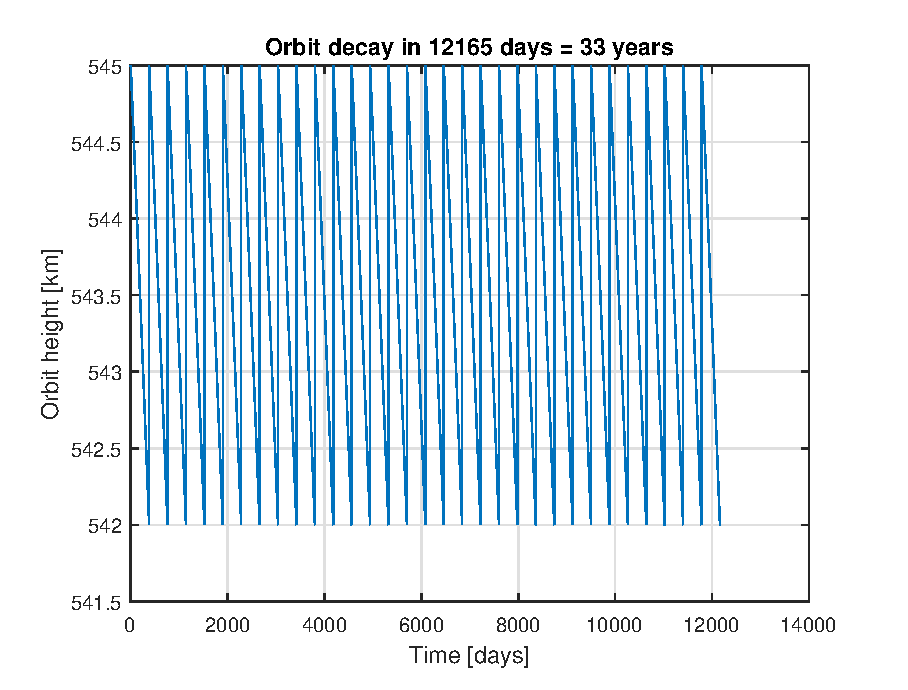
\includegraphics[scale=1]{ThrustersDrag/thrust3km.eps}}
\caption{Height variation of the satellite}
\label{fig:hohmann3km}
\end{figure}

Figure \ref{fig:hohmann3km} is an example of the height variation of the satellite using the Hohmann maneuver to reach the maximum height once the satellite is in the minimum height. The results of this maneuver are:

\begin{table}
\begin{center}
\begin{tabular}{ | l | l | }
\hline
Maximum height & 545 km \\
\hline
Minimum height & 542 km \\
\hline
Number of Hohmann Maneuvers & 32 \\
\hline
Maximum $\Delta$V\textsubscript{1} & 0.8237 m/s \\
\hline
Maximum $\Delta$V\textsubscript{2} & 0.8236 m/s \\
\hline
Total $\Delta$V Budget & 52.7116 m/s \\ 
\hline 
Propellant mass & 10 g \\
\hline
Lifetime of the satellite & 33.3288 years \\
\hline
\end{tabular}
\caption{Station-Keeping with Thrusters Simulation 1 Results}
\end{center}
\end{table}

\noindent
Since the thruster used is an ion thruster, the specific impulse is big, and the mass propellant is very low. In this case, the variation of height due to the orbit decay is approximately 3 km per year, so the thruster needs to do a Hohmann maneuver per year. With only 10 g of propellant, the lifetime of the satellite is over 30 years.

\begin{figure}[h]
\centerline{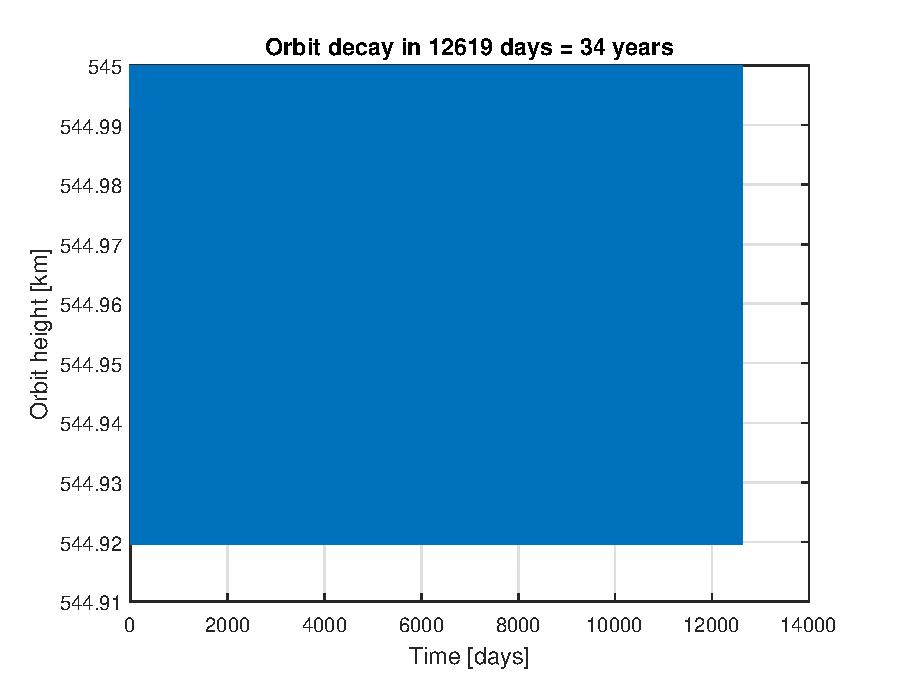
\includegraphics[scale=1]{ThrustersDrag/thrust80m.eps}}
\caption{Height variation of the satellite with a more restrictive minimum height}
\label{fig:hohmann80m}
\end{figure}

Figure \ref{fig:hohmann80m} is another example of the Hohmann maneuver with the same amount of propellant but with a more restrictive range of operational heights, only 80 m. It should have the same shape as Figure \ref{fig:hohmann3km}, but since a lot of maneuvers are applied, the lines have overlapped. The characteristics of this maneuver are:

\begin{table}
\begin{center}
\begin{tabular}{ | l | l | }
\hline
Maximum height & 545 km \\
\hline
Minimum height & 544.92 km \\
\hline
Number of Hohmann Maneuvers & 1200 \\
\hline
Maximum $\Delta$V\textsubscript{1} & 0.0221 m/s \\
\hline
Maximum $\Delta$V\textsubscript{2} & 0.0221 m/s \\
\hline
Total $\Delta$V Budget & 52.7570 m/s \\ 
\hline 
Propellant mass & 10 g \\
\hline
Lifetime of the satellite & 34.5726 years \\
\hline
\end{tabular}
\caption{Station-Keeping with Thrusters Simulation 2 Results}
\end{center}
\end{table}

\noindent
Comparing these results with the previous ones, it can be seen that with a more restrictive range of heights, the lifetime of the satellite is practically the same. The velocity increments are lower because the difference in the heights is extremely low, but at the same time, the satellite reaches before the minimum height and the maneuvers needed to maintain the satellite in this range are many more than on the other case. Since the $\Delta$V budget is practically the same in both cases, it can be assured that the only difference between them is the number of maneuvers computed.
\paragraph{}
As mentioned earlier, the results obtained are for a Hohmann maneuver when in reality the satellite will compute a low-thrust maneuver, that requires less velocity increments and less propellant. In conclusion, taking into account these results, it can be stated that the lifetime of the satellite will not be determined by its orbit decay but for the failure of its systems or other external causes. It can also be assured that the satellite is capable of carrying enough propellant to maintain its altitude and to compute other maneuvers if necessary.